\documentclass[12pt, letterpaper, twoside]{article}
\usepackage[utf8]{inputenc}
\usepackage[english,russian]{babel}
\usepackage{tikz}  
\usetikzlibrary{graphs}
\usepackage{amsmath}
\usepackage{amssymb}
\DeclareMathOperator*{\argmin}{argmin} 
\graphicspath{ {./} }
\usepackage{listings}

\title{First document}
\author{Serhy Makarenko \thanks{funded by the ShareLaTeX team}}
\date{December 2018}

\begin{document}
	
\begin{titlepage}
	\begin{center}
		\large



		\vspace{0.5cm}
				Міністерство освіти та науки України\\
		Національний Технічний Університет України\\
		«Київський Політехнічний Інститут»
\\
	
		\vspace{0.25cm}
		
	Фізико – технічний інститут


		\vfill
		
		\textsc{Лабораторна робота №2}\\[5mm]
		
		{\LARGE «Метод спряжених градієнтів»}
		\bigskip
		
	\end{center}
	\vfill
	
	\newlength{\ML}
	\settowidth{\ML}{«\underline{\hspace{0.7cm}}» \underline{\hspace{2cm}}}
	\hfill\begin{minipage}{0.3\textwidth}
		Виконали:\\
		 Студенти 4 курсу\\
		 Групи ФI-51\\
		 Макаренко Сергій\\
		 Скiрдiн Євгенiй\\
		 Сiтко Дарина\\
		 Сiмакова Катерина\\
	
	\end{minipage}%
	\bigskip
	
	\hfill\begin{minipage}{0.3\textwidth}
		Перевірив:\\
		Данилов В.Я
	\end{minipage}%
	\vfill
	
	\begin{center}
		Київ, 2018 р.
	\end{center}
\end{titlepage}
	


\begin{center}
	Теоретичні відомості
\end{center}


Нехай f(x) – випукла диференційована в усьому просторі \ функція і треба знайти її точку мінімуму.

Тобто знайти  $\displaystyle \argmin_{x\in R^{n}} \ f_{0}( x)$ для \ \ заданої \ \ неперервно \ диференційованої \ функції \ $\displaystyle f_{0} :R^{n}\rightarrow R^{1}$
\vspace{0.9cm}



Алгоритм:
\begin{enumerate}
	\item Вибрати \ \ довільне \ \ початкове \ \ наближення $\displaystyle x^{0} \in R^{n}$ , \ натуральне \ число \ $\displaystyle \tau \geqslant n$ ( $\displaystyle \tau $ – момент \ відновлення), покласти \ $\displaystyle k=0$.
	\item Обчислити $\displaystyle \nabla f_{0}\left( x^{0}\right)$ і \ покласти \ $\displaystyle g^{0} =-\nabla f_{0}\left( x^{0}\right)$ , $\displaystyle h^{0} =-\nabla f_{0}\left( x^{0}\right)$.
	\item Обчислити \ \ кроковий \ \ множник $\displaystyle \rho _{k}$ , що задовольняє \ умову $\displaystyle f_{0}\left( x^{k} +\rho _{k} h^{k}\right) =\min_{\rho \geqslant 0} f_{0}\left( x^{k} +\rho h^{k}\right)$.
	\item Обчислити наближення: $\displaystyle x^{k+1} =x^{k} +\rho h^{k}$.
	\item Обчислити $\displaystyle \nabla f_{0}\left( x^{k+1}\right)$ і \ покласти \ $\displaystyle g^{k+1} =-\nabla f_{0}\left( x^{k+1}\right)$
	\item Якщо \ \ $\displaystyle g^{k+1} =0$ , \ то \ покласти \ $\displaystyle x^{*} =x^{k+1}$ і \ завершити обчислення, \ інакше \ перейти \ на \ крок \ 7.
	\item Обчислити \ коефіцієнт $\displaystyle \beta _{k} =\omega \left(\dfrac{k+1}{\tau }\right)\dfrac{\left( g^{k+1} -g^{k} ,g^{k+1}\right)}{\left( g^{k} ,g^{k}\right)}$ , де \\ $\displaystyle \omega ( t) =\begin{cases}
	0, & \ if\ \ t-integer\ \\
	1, & else
	\end{cases}$
	\item Обчислити \ вектор $\displaystyle h^{k+1} =g^{k+1} +\beta _{k} h^{k} \ .$
	\item  Покласти \ $\displaystyle k=k+1$ і \ перейти \ на \ крок \ 3.
\end{enumerate}
\clearpage
Блок - схема алгоритму:\\


\tikzset{every picture/.style={line width=0.75pt}} %set default line width to 0.75pt        

\begin{tikzpicture}[x=0.75pt,y=0.75pt,yscale=-1,xscale=1]
%uncomment if require: \path (0,649.25); %set diagram left start at 0, and has height of 649.25

%Shape: Rectangle [id:dp9669737833751013] 
\draw   (194.5,20) -- (436.5,20) -- (436.5,60) -- (194.5,60) -- cycle ;
%Shape: Rectangle [id:dp332998149296713] 
\draw   (137.71,90.64) -- (271,90.64) -- (271,147.61) -- (137.71,147.61) -- cycle ;
%Straight Lines [id:da6961868815017703] 
\draw    (212.67,60.55) -- (212.51,86.6) ;
\draw [shift={(212.5,88.6)}, rotate = 270.34000000000003] [color={rgb, 255:red, 0; green, 0; blue, 0 }  ][line width=0.75]    (10.93,-3.29) .. controls (6.95,-1.4) and (3.31,-0.3) .. (0,0) .. controls (3.31,0.3) and (6.95,1.4) .. (10.93,3.29)   ;

%Straight Lines [id:da05276189258048014] 
\draw    (272.5,113.92) -- (323.5,114.57) ;
\draw [shift={(325.5,114.6)}, rotate = 180.74] [color={rgb, 255:red, 0; green, 0; blue, 0 }  ][line width=0.75]    (10.93,-3.29) .. controls (6.95,-1.4) and (3.31,-0.3) .. (0,0) .. controls (3.31,0.3) and (6.95,1.4) .. (10.93,3.29)   ;

%Shape: Rectangle [id:dp01285605895775288] 
\draw   (121,225) -- (191,225) -- (191,265) -- (121,265) -- cycle ;
%Shape: Rectangle [id:dp6404040763905939] 
\draw   (211.17,327) -- (452.17,327) -- (452.17,409.25) -- (211.17,409.25) -- cycle ;
%Flowchart: Preparation [id:dp36907176624835236] 
\draw   (219.5,245.96) -- (239.19,227) -- (304.81,227) -- (324.5,245.96) -- (304.81,264.92) -- (239.19,264.92) -- cycle ;
%Straight Lines [id:da8410235228245763] 
\draw    (321,409.25) -- (320.54,432.6) ;
\draw [shift={(320.5,434.6)}, rotate = 271.13] [color={rgb, 255:red, 0; green, 0; blue, 0 }  ][line width=0.75]    (10.93,-3.29) .. controls (6.95,-1.4) and (3.31,-0.3) .. (0,0) .. controls (3.31,0.3) and (6.95,1.4) .. (10.93,3.29)   ;

%Straight Lines [id:da04627637104225346] 
\draw    (347.5,180.96) -- (319.5,180.62) ;
\draw [shift={(317.5,180.6)}, rotate = 360.68] [color={rgb, 255:red, 0; green, 0; blue, 0 }  ][line width=0.75]    (10.93,-3.29) .. controls (6.95,-1.4) and (3.31,-0.3) .. (0,0) .. controls (3.31,0.3) and (6.95,1.4) .. (10.93,3.29)   ;

%Shape: Rectangle [id:dp16853315795314727] 
\draw   (244,437) -- (385,437) -- (385,471.25) -- (244,471.25) -- cycle ;
%Straight Lines [id:da6249136791705401] 
\draw    (411.5,131.92) -- (411.5,158.6) ;
\draw [shift={(411.5,160.6)}, rotate = 270] [color={rgb, 255:red, 0; green, 0; blue, 0 }  ][line width=0.75]    (10.93,-3.29) .. controls (6.95,-1.4) and (3.31,-0.3) .. (0,0) .. controls (3.31,0.3) and (6.95,1.4) .. (10.93,3.29)   ;

%Shape: Rectangle [id:dp28894658884603297] 
\draw   (167,160) -- (314.5,160) -- (314.5,198.92) -- (167,198.92) -- cycle ;
%Straight Lines [id:da413212276195993] 
\draw    (385.5,454.92) -- (413.5,455.55) ;
\draw [shift={(415.5,455.6)}, rotate = 181.3] [color={rgb, 255:red, 0; green, 0; blue, 0 }  ][line width=0.75]    (10.93,-3.29) .. controls (6.95,-1.4) and (3.31,-0.3) .. (0,0) .. controls (3.31,0.3) and (6.95,1.4) .. (10.93,3.29)   ;

%Straight Lines [id:da8103348891124106] 
\draw    (276.5,265.92) -- (277.47,323.92) ;
\draw [shift={(277.5,325.92)}, rotate = 269.05] [color={rgb, 255:red, 0; green, 0; blue, 0 }  ][line width=0.75]    (10.93,-3.29) .. controls (6.95,-1.4) and (3.31,-0.3) .. (0,0) .. controls (3.31,0.3) and (6.95,1.4) .. (10.93,3.29)   ;

%Shape: Rectangle [id:dp9591886070808326] 
\draw   (326.5,90) -- (529.83,90) -- (529.83,132.25) -- (326.5,132.25) -- cycle ;
%Straight Lines [id:da7699410526786881] 
\draw    (275.5,198.92) -- (275.5,222.6) ;
\draw [shift={(275.5,224.6)}, rotate = 270] [color={rgb, 255:red, 0; green, 0; blue, 0 }  ][line width=0.75]    (10.93,-3.29) .. controls (6.95,-1.4) and (3.31,-0.3) .. (0,0) .. controls (3.31,0.3) and (6.95,1.4) .. (10.93,3.29)   ;

%Shape: Rectangle [id:dp5747289392708681] 
\draw   (350.5,163) -- (472.5,163) -- (472.5,203) -- (350.5,203) -- cycle ;
%Shape: Rectangle [id:dp07998355067183904] 
\draw   (419.5,433) -- (516,433) -- (516,473) -- (419.5,473) -- cycle ;
%Straight Lines [id:da6876523832686033] 
\draw    (219.5,245.96) -- (196.5,245.63) ;
\draw [shift={(194.5,245.6)}, rotate = 360.82] [color={rgb, 255:red, 0; green, 0; blue, 0 }  ][line width=0.75]    (10.93,-3.29) .. controls (6.95,-1.4) and (3.31,-0.3) .. (0,0) .. controls (3.31,0.3) and (6.95,1.4) .. (10.93,3.29)   ;

%Straight Lines [id:da31787197431448055] 
\draw    (505.5,431.92) -- (503.51,135.6) ;
\draw [shift={(503.5,133.6)}, rotate = 449.62] [color={rgb, 255:red, 0; green, 0; blue, 0 }  ][line width=0.75]    (10.93,-3.29) .. controls (6.95,-1.4) and (3.31,-0.3) .. (0,0) .. controls (3.31,0.3) and (6.95,1.4) .. (10.93,3.29)   ;

%Straight Lines [id:da1993576384051926] 
\draw    (150.5,264.92) -- (150.81,297.55) ;
\draw [shift={(150.83,299.55)}, rotate = 269.45] [color={rgb, 255:red, 0; green, 0; blue, 0 }  ][line width=0.75]    (10.93,-3.29) .. controls (6.95,-1.4) and (3.31,-0.3) .. (0,0) .. controls (3.31,0.3) and (6.95,1.4) .. (10.93,3.29)   ;

%Shape: Rectangle [id:dp10817897950938749] 
\draw   (132.5,301) -- (173.5,301) -- (173.5,321.92) -- (132.5,321.92) -- cycle ;

% Text Node
\draw (310,40) node   {$x^{0} =\overline{0} ,\ \tau =n+1,\ k=0$};
% Text Node
\draw (203.45,119.13) node   {$ \begin{array}{l}
	g^{0} =-\nabla f_{0}\left( x^{0}\right)\\
	h^{0} =-\nabla f_{0}\left( x^{0}\right)
	\end{array}$};
% Text Node
\draw (156,241) node   {$x^{*} =x^{k+1}$};
% Text Node
\draw (335,373) node   {$\beta _{k} =\omega \left(\dfrac{k+1}{\tau }\right)\dfrac{\left( g^{k+1} -g^{k} ,g^{k+1}\right)}{\left( g^{k} ,g^{k}\right)}$};
% Text Node
\draw (271,245) node  [align=left] {$\displaystyle g^{k+1} =0?$};
% Text Node
\draw (296,283) node  [align=left] {Нi};
% Text Node
\draw (313,454) node   {$h^{k+1} \ =g^{k+1} +\beta _{k} h^{k}$};
% Text Node
\draw (244,178) node   {$g^{k+1} =-\nabla f_{0}\left( x^{k+1}\right)$};
% Text Node
\draw (211,233) node  [align=left] {Так};
% Text Node
\draw (429,108) node   {$\rho _{k} =argmin_{\rho } f_{0}\left( x^{k} +\rho h^{k}\right)$};
% Text Node
\draw (417,181) node   {$x^{k+1} =x^{k} +\rho _{k} h^{k} \ .$};
% Text Node
\draw (463,454) node   {$k=k+1$};
% Text Node
\draw (153,313) node  [align=left] {end};


\end{tikzpicture}

\clearpage
\lstinputlisting[language=Python]{lab.py}
Результати: $\displaystyle x_{1} =-0.5;\ x_{2} =0;\ f\left(\overline{x}\right) =-0.25$ \\
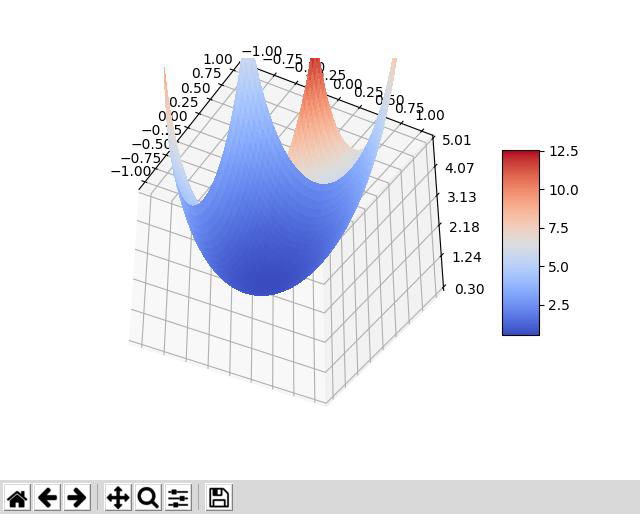
\includegraphics[scale=0.7]{pic1.png}



\end{document}

